        \clearpage
        \begin{figure*}[ht]
            \pdfbookmark[2]{ID 07}{figure_id_07}
        	\centering
            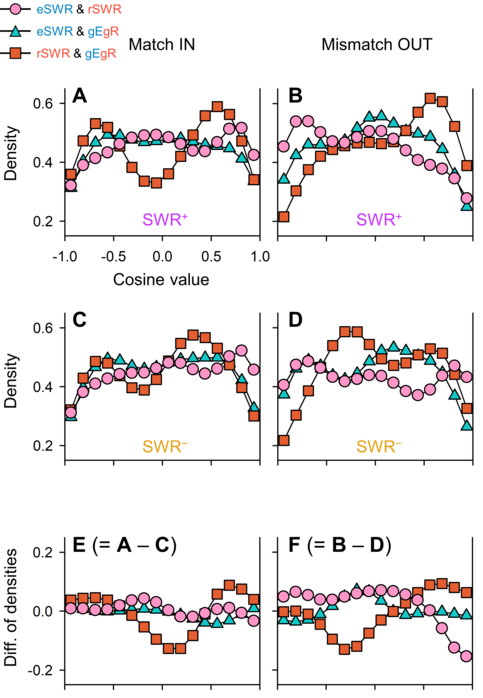
\includegraphics[width=0.5\textwidth]{./src/figures/.png/Figure_ID_07.png}
        	\caption{\textbf{
Neural Trajectory Directions during SWRs: Encoding and Retrieval States
}
\smallskip
\\
\textbf{\textit{A--B}} Kernel density estimation (KDE) distributions of $\protect\overrightarrow{{\mathrm{eSWR^+}}} \cdot \protect\overrightarrow{{\mathrm{rSWR^+}}}$ (\textit{pink circles}), $\protect\overrightarrow{{\mathrm{eSWR^+}}} \cdot \protect\overrightarrow{{\mathrm{g_{E}g_{R}}}}$ (\textit{blue triangles}), and $\protect\overrightarrow{{\mathrm{rSWR^+}}} \cdot \protect\overrightarrow{{\mathrm{g_{E}g_{R}}}}$ (\textit{red rectangles}) are shown for Match IN (\textit{A}) and Mismatch OUT tasks (\textit{B}). \textbf{\textit{C--D}} Display the corresponding distributions of $\mathrm{SWR^-}$ replacing those of $\mathrm{SWR^+}$ in \textit{A} and \textit{B}. \textbf{\textit{E--F}} Illustrate the discrepancies in the distributions of $\mathrm{SWR^+}$ and $\mathrm{SWR^-}$, highlighting the SWR components (\textit{E} = \textit{C} $-$ \textit{A}; \textit{F} = \textit{D} $-$ \textit{B}). Observe the biphasic distributions of $\protect\overrightarrow{{\mathrm{rSWR^-}}} \cdot \protect\overrightarrow{{\mathrm{g_{E}g_{R}}}}$, indicating fluctuations between the encoding and retrieval states throughout the Sternberg task. Additionally, contrasting directionality between $\protect\overrightarrow{{\mathrm{eSWR^+}}}$ and $\protect\overrightarrow{{\mathrm{rSWR^+}}}$ was noticed (\textit{pink circles}) in the Mismatch OUT task, but was absent in the Match IN task (\textbf{\textit{E--F}}). Lastly, transitions from the retrieval to the encoding states were prominent in the SWR components in both the Match IN and Mismatch OUT tasks (\textit{red rectangles} in \textit{E} and \textit{F}).
}
% width=0.5\textwidth
        	\label{fig:07}
        \end{figure*}
